
\chapter{Metodologia}

Para a execução deste projeto, optou-se pelo uso de componentes amplamente disponíveis no mercado a relativamente baixo
custo, bem como software disponível gratuitamente no site do fabricante. Essas escolhas visam facilitar a
reproducibilidade do projeto, bem como tornar o resultado final do projeto mais eficiente, produzindo o resultado
desejado com o menor custo. 

Um outro fator relevante que impactou a escolha dos componentes a serem utilizados no projeto é a compatibilidade entre
eles - seja ela mecânica, eletrônica ou mesmo de software. Diferentemente de uma solução completa oferecida por
um só fabricante, em que há garantia de operação harmoniosa entre os componentes, este trabalho envolveu a composição de
diferentes partes, pelo que se tornou necessário avaliar a viabilidade de se utilizar todas elas em conjunto.

Ainda assim, dada a necessidade de se utilizar peças com formatos e dimensões específicas para a aplicação em questão,
optou-se também pelo uso de técnicas de impressão 3D. Essa decisão é compatível com o objetivo geral de baixos custos, e
também resolve problemas relacionados à montagem mecânica.


\section{Hardware}
A aquisição dos componentes de hardware empregados neste projeto se deu, em boa parte, por meio de lojas importadoras de
componentes. Optou-se por componentes de baixo custo e, ao mesmo tempo, comumente utilizados em projetos dessa natureza,
a fim de se ter amplo apoio da comunidade na resolução de eventuais problemas encontrados no desenvolvimento da solução.
A tabela \ref{custos} apresenta os custos de cada componente de hardware adquirido para uso exclusivo neste projeto
(excluindo, portanto, equipamentos empregados mas não utilizados apenas nele, como a impressora 3D).


\begin{quadro}[htb]
	\caption{Lista de componentes, materiais e seus custos - valores em reais (R\$) \label{custos}}
	 \begin{tabular}{|c|c|c|c|}
		\hline
		\textbf{Componente ou Material} & \textbf{Valor unitário} & \textbf{Quant} & \textbf{Valor Total} \\ \hline
		Driver Ponte H L298N \cite{l298n_produto} &  22,90 & 3 &  68,70   \\ \hline
		Motor DC 6V 210 RPM \cite{motor_dc_6v_produto} &  90,00 & 3 &  270,00   \\ \hline
		Filamento PLA \cite{filamento_pla_produto} &  99,99 & 1 &  99,99   \\ \hline
		Kit 4 rodas Omnidirecional \cite{omin_wheel_produto} &  131,35 & 1 &  131,35   \\ \hline
		Kit 4 peças eixo roda \cite{omin_wheel_produto} &  42,15 & 1 &  42,15   \\ \hline
		STM32 (microcontrolador) \cite{stm32_produto} &  46,90 & 1 &  46,90   \\ \hline
		Bateria selada 6V \cite{bateria_6v_produto} &  69,90 & 1 &  69,90  \\ \hline
		Powerbank &  119,90 & 1 &  119,90   \\ \hline
		Paquímetro  &  49,90 & 1 &  49,90   \\ \hline
		Ferro de solda &  43,20 & 1 &  43,20   \\ \hline
		Solda &  12,99 & 1 &  12,99   \\ \hline
		Conector mjjst macho &  4,90 & 3 &  14,70   \\ \hline
		Conector mjjst femea &  4,90 & 3 &  14,70   \\ \hline
		Garra jacaré &  1,65 & 2 &  3,30   \\ \hline
		Driver Ponte H DTV8833 \cite{drv8833_produto} &  15,00 & 3 &  45,00   \\ \hline
		Módulo Bluetooth \cite{hc05_produto} &  35,00 & 1 &  35,00   \\ \hline
		Mini Protoboard &  5,00 & 2 &  10,00   \\ \hline
		Protoboard 830 &  16,00 & 1 &  16,00   \\ \hline
		Jumper macho-macho &  8,00 & 1 &  8,00   \\ \hline
		Pasta de solda &  14,99 & 1 &  14,99   \\ \hline
		Sugador de solda &  12,99 & 1 &  12,99   \\ \hline	
		\textbf{CUSTO TOTAL} & & & \textbf{ 1.129,66}   \\ \hline
	\end{tabular}
\end{quadro}

\subsection{Componentes eletrônicos}

\subsubsection{Motor de passo}

Para a execução deste projeto, foi pensado inicialmente o uso de motores DC,  devido a facilidade de uso.
Como os motores DC variam a velocidade com base na tensão disponível, tornando o acionamento simples.
Porém o controle de velocidade é mais complexo, fazendo o uso de encoders.
A leitura dos resultados do encoders possuem muitos ruidos de medição e variam muito com a frequência de amostragem, 
mas remover os ruidos de alta frequência do sinal possa ser resolvido usando um algorítimo de filtro passa baixa discreto.
Porém os motores DC tem a limitação de trabalharem em uma faixa de rpm específica, podendo o motor não alcançar um rpm mínimo desejado.
Um motor de 6v/210 RPM usado tinha baixo torque a baixas velocidades, além de precisar de uma corrente de partida mais alta do que a tensão inicial fornecia.
Trocar por motores de menor velocidade acabaria tendo o problema de não ser possível alçarem um velocidade mais alta quando necessário.
Para usar um motor DC com uma boa variação de velocidade, seria necessário usar um conjunto de engrenagens para obter o rpm desejado sem grandes perdas de torque nos motores
e sem problemas de corrente de partida insuficiente.

Devido essas limitações se optou por motores de passo,  nema 17 bipolar, de uso padrão em impressoras 3D.
A escolha foi motivada pela facilidade de aquisição e maior disponibilidade no mercado, tornando o preço mais baixo do que motores DC,
Em média os valores de um Nema 17 chegam a metade do valor de um motor DC de baixo RPM.
Outro motivo que levou a escolha, foi o fato de serem motores de reposição de uma impressora 3D usada no projeto.

Pelo fato de motor de passo ser controlado em passos por segundo, o controle de velocidade é mais fácil,
e as possíveis variações de rpm ocorrem a nível de ciclos do microcontrolador.

Porém motores de passo exigem um cuidado maior, além de exigem uma alimentação maior, de 12v a 24v, os uso dos drivers para motor de passo exigem um maior cuidado na montagem.

\begin{figure}[htb]
	\centering
	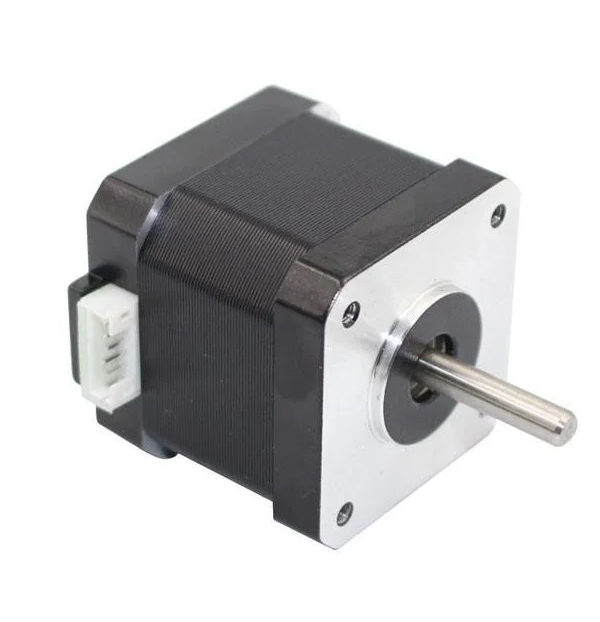
\includegraphics[width=0.7\textwidth]{figures/JK42HS40_1704_13A}
	\caption{Motor de passo Nema 17 \cite{motor_dc_6v_encoder}}
\end{figure}

\begin{quadro}[htb]
\caption{\label{Especificacoes_motordc_6v}Especificações do motor DC 6V}
	 \begin{tabular}{|c|c|c|c|}
		\hline
		\textbf{Especificação} & \textbf{Valor} \\ \hline
		Corrente por fase & 1.7A  \\ \hline
		Torque nomimal  & 4.2 KGF (~46 N) \\ \hline
		Angulo de passo & 1.8° \\ \hline
		Polaridade & bipolar \\ \hline
	\end{tabular}
	\fonte{\cite{chinhai_motor}}
\end{quadro}


Outro desafio do motor de passo é idenfiticar as fases, pois cada fabricante pode ter uma ordem diferente dos pinos de saida do motor.
Para idenfiticar quais pinos compõem cada fase, bastou verificar com o multimetro quais fases estavam em curto.
Restando identicar somente o pontos A e B de cada fase de acordo com o diagrama a seguir.

\begin{figure}[htb]
	\centering
	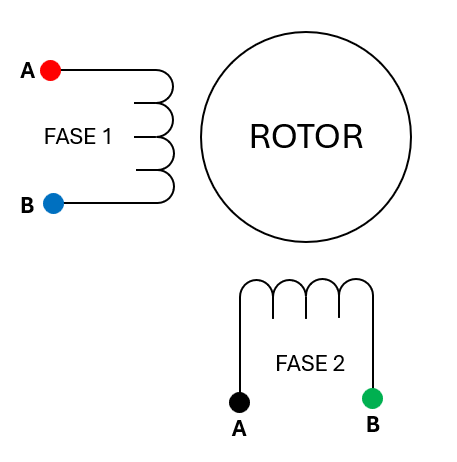
\includegraphics[width=0.7\textwidth]{figures/motor_wiring}
	\caption{Motor de passo - Fases Bipolar \cite{motor_dc_6v_encoder}}
\end{figure}

Para identificar quais eram os pontos A e B de cada fase, foi necessário um processo de tentantiva e erro,
para relacionar o diagrama de fases com os pinos do motor, e o resultado esta ilustrado na figura \ref{nema_pinout}

\begin{figure}[htb]
	\centering
	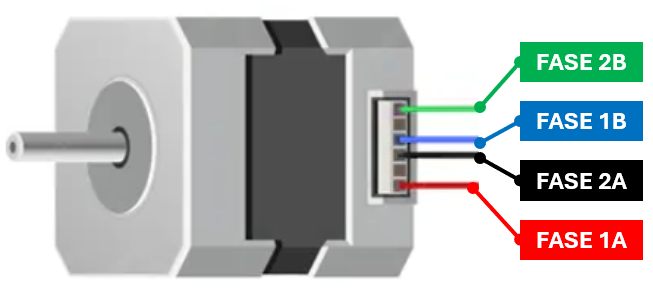
\includegraphics[width=0.7\textwidth]{figures/motor_pinout}
	\caption{Motor de passo - Idetificação dos pinos  \cite{motor_dc_6v_encoder}}
	\label{nema_pinout}
\end{figure}



\subsubsection{Driver de Motor}

Diferente de um driver de motor DC, como o L289N e o DRV8833, que rececem um sinal PWM e convertem propocionalmente
para o sinal de tensão a ser aplicado no motor,  os driver de motor de passo são responsáveis por aplicar uma corrente constante, independende da tensão de alimentação.
sendo essa podendo variar de acordo com os limites dos motores e do próprio driver,  por convensão, para um Nema 17, é comnum se trabalhar com uma alimentação
de 12v a 24v.

O driver DRV8825 exige alguns cuidados, alguns informados em documentação e outros não.
Um dos cuidado a ser informado é o ajuste do Vref, nas documentações é dito que é necessário apenas ligar a alimentação dos motores e o ground do microcontrolador
porém em vários testes, alguns drivers pararam de funcionar,  foi então encontrado em fóruns que é recomendado que a carga (o motor) esteja ligado durante esse processo de ajuste do Vref
e que e nenhuma hipotese o driver deve ser alimentado sem que a carga esteja conectada.


\begin{figure}[htb]
	\centering
	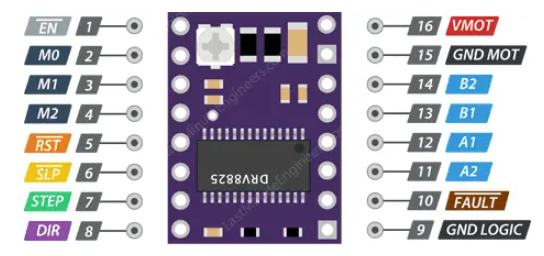
\includegraphics[width=0.7\textwidth]{figures/DRV8825}
	\caption{Driver Ponte H DVR8833 \cite{DRV8833_image}}
\end{figure}


\subsubsection{Microcontrolador}

Inicialmente foi escolhido o STM32F103C8, porém a comunicação serial via microusb não pode ser usada ao mesmo tempo que
a alimentação de 3.3v do gravador ST-link. isso pode causar danos no controlador. Por causa dessa limitação foi escolhido o ESP32 DevKit v1.
Embora  quantidade de pinos disponíveis seja menor, não será necessário o uso de pinos de comunicação serial para usar com um módulo bluetooth,
já que o ESP32 já possui bluetooth integrado.

De acordo com o datasheet do ESP32 \cite{esp32_datasheet} e a análises disponíveis online de entusiastas do uso do ESP32 \cite{esp32_reference},
existem alguns pinos recomendados para se usar, alguns que requerem atenção no uso, e outros que recomendam evitar.

\begin{figure}[htb]
	\centering
	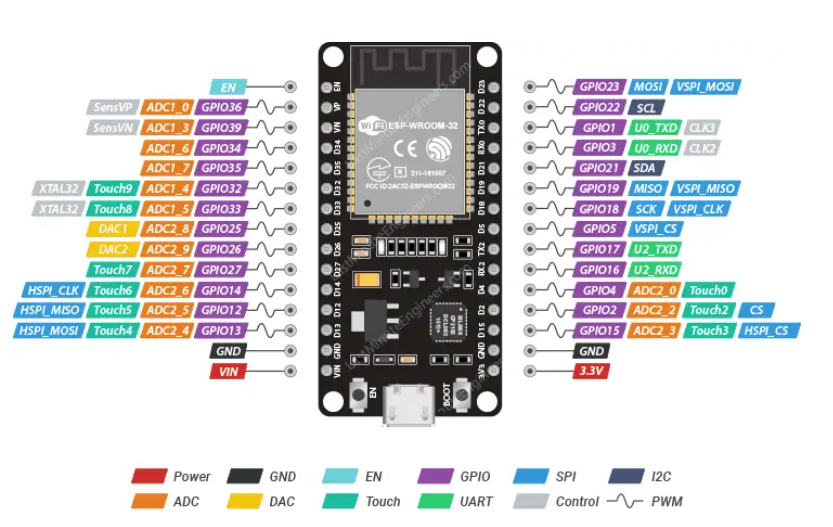
\includegraphics[width=1.0\textwidth]{figures/esp32_pinout}
	\caption{Diagrama de pinos do ESP32 Devkit v1 \cite{esp32_reference}}
\end{figure}


\begin{figure}[htb]
	\centering
	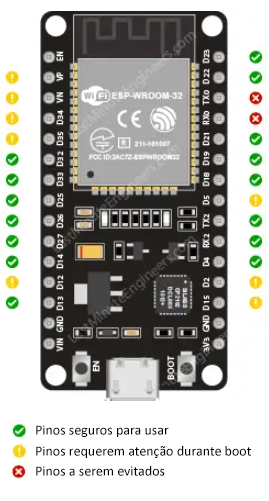
\includegraphics[width=0.35\textwidth]{figures/esp32_pinout_ref}
	\caption{Recomendação de uso dos pinos do ESP32 Devkit v1 \cite{esp32_reference}}
\end{figure}


\subsubsection{Alimentação - ESP32}

Para alimentação do ESP32, pode usar tanto uma bateria de 5v ou 3.3v, pois possui dois pinos para alimentação: 

\subsubsubsection{Pino de 5v não regulado}

Fontes divergem em relação à tensão máxima (\cite{esp32_reference_power_supply_1}, \cite{esp32_reference_power_supply_2}),
que pode ser usada, porém, a maioria concorda em manter de 6v a 7v.

\subsubsubsection{Pino de 3.3v regulado}
Esse pino pode receber no máximo 3.3v, podendo funcionar entre 3.1v e 3.3v sem problema.

\subsubsubsection{micro USB}
Essa opção permite usar um powerbank, porém o conector do ESP32 é um Micro-USB B, modelo que usa protocolo USB 2.0, que pode fornece apenas a 500mA a 5v \cite{micro_usb_b}.
500mA É suficiente para alimentar o ESP32, que pode consumir até 260mA \cite{esp_max_current}.
Porem um powerbank pode ser uma solução muito ineficiente do ponto de vista energético, os modelos populares possuem baterias de lítio de 3.7v, que é convertido para 5v,
e posteriormente dentro do ESP32 a tensão é convertida novamente para 3.3v. Apenas no modelo PN-952 da CNHPineng sai de 5000mAh a 3.7v  para 3160mAh a 5v,
podendo novamente perder mais corrente por hora ao ser convertido para 3.3v no ESP32

\subsubsection{Motores de passo}

Os motores de passo NEMA 17 podem ser alimentados, através do driver, com 12v a 24v.
Observando a possibilidade de uma bateria de 12v/24v ficar sem uso depois do projeto,
e considerando que ferramentas elétricas possuem baterias padronizadas de 12v/18v/36V, foi considerando utilizar 3 baterias de 12v da bosch, que já estavam disponíveis para uso.
Cada bateria tem tensão nominal de 12v a 2Ah, do modelo GBA, que são usadas em aspirador de pó, esmerilhadeiras, furadeiras, plainas e serras circulares.


https://www.bosch-professional.com/br/pt/products/gba-12v-max-2-0ah-1600A0021D
https://www.bosch-professional.com/br/pt/products/gas-12v-06019E3000
https://www.bosch-professional.com/br/pt/products/gwg-12v-50-s-06013A70E0


\subsection{Fabricação e montagem}
O chassi e demais peças foram fabricados por meio de impressão 3D, usando filamento de PLA (ácido poliáctico). As
peças foram projetadas no AutoCAD, e posteriormente modeladas em 3D com o SolidWorks. A geometria do modelo
resultante de cada peça foi convertida em código G para uma impressora 3D por meio do software UltiMaker Cuda. Por
fim, a impressão das peças foi realizada em uma impressora Ender 3 S1 Pro.



% \subsection{Joystick de controle}
% Um joystick de 3 eixos para controlar o robô para testar a cinemática de movimento.
% {\color{red} É necessário aqui especificar o modelo utilizado e descrever características.}

% \subsection{Sensores}
% {\color{red} Esta subseção deve descrever os sensores utilizados e também sua finalidade.}

% \subsection{Dispositivos de comunicação}
% {\color{red} Esta subseção deve descrever os dispositivos de comunicação utilizados (Wi-fi, Bluetooth, etc) e também sua
% finalidade.}

% \subsection{Calibração de parâmetros}
% {\color{red} Caso haja necessidade de calibração de parâmetros de alguns dos componentes utilizados (sensibilidade de
% sensores, histerese de componentes mecânicos, taxa de comunicação de dispositivos, etc), os procedimentos devem ser
% descritos nesta subseção.}

\section{Software}
Para controlar o robô, inicialmente foi pensando em usar uma aplicação drag\&drop para criar um app andriod que envia dados via bluetooth serial.
Porem realizando um benchmark de outros app disponíveis para interações bluetooth com arduino optamos por usar dois desses app e usar de uma maneira diferente.


\subsection{Programação do microcontrolador}

Nesta aplicação, o microcontrolador contém é responsável por coordenar a operação do robô. Por essa razão, foi
necessário programar tal funcionalidade em sua memória. Neste processo, foi necessário configurar os diferentes pinos de
entrada segundo suas capacidades e o uso desejado no projeto, bem como implementar o processamento dos sinais de entrada
(referentes à velocidade dos motores) e a produção de saída (valores a serem enviados como variável manipulada para os
motores do robô). É também do microcontrolador a tarefa de interpretar os comandos recebidos via Bluetooth do próprio microcontrolador
e convertê-los em sinal de controle.

\subsection{Aplicativo Android}

O aplicativo Arduino Bluetooth Controller possui uma opção em que o aplicativo envia uma 'string' representando as cores RGB em 'int8'.
por exemplo,  vermelho seria '255000000' (r=255, g=0, b=0). E a interface é o modelo de cor HSV em 2 dimensões de ponta cabeça,
figura \ref{arduino_bluetooth_controller_hsl_model}.


\begin{figure}[htb]
	\centering
	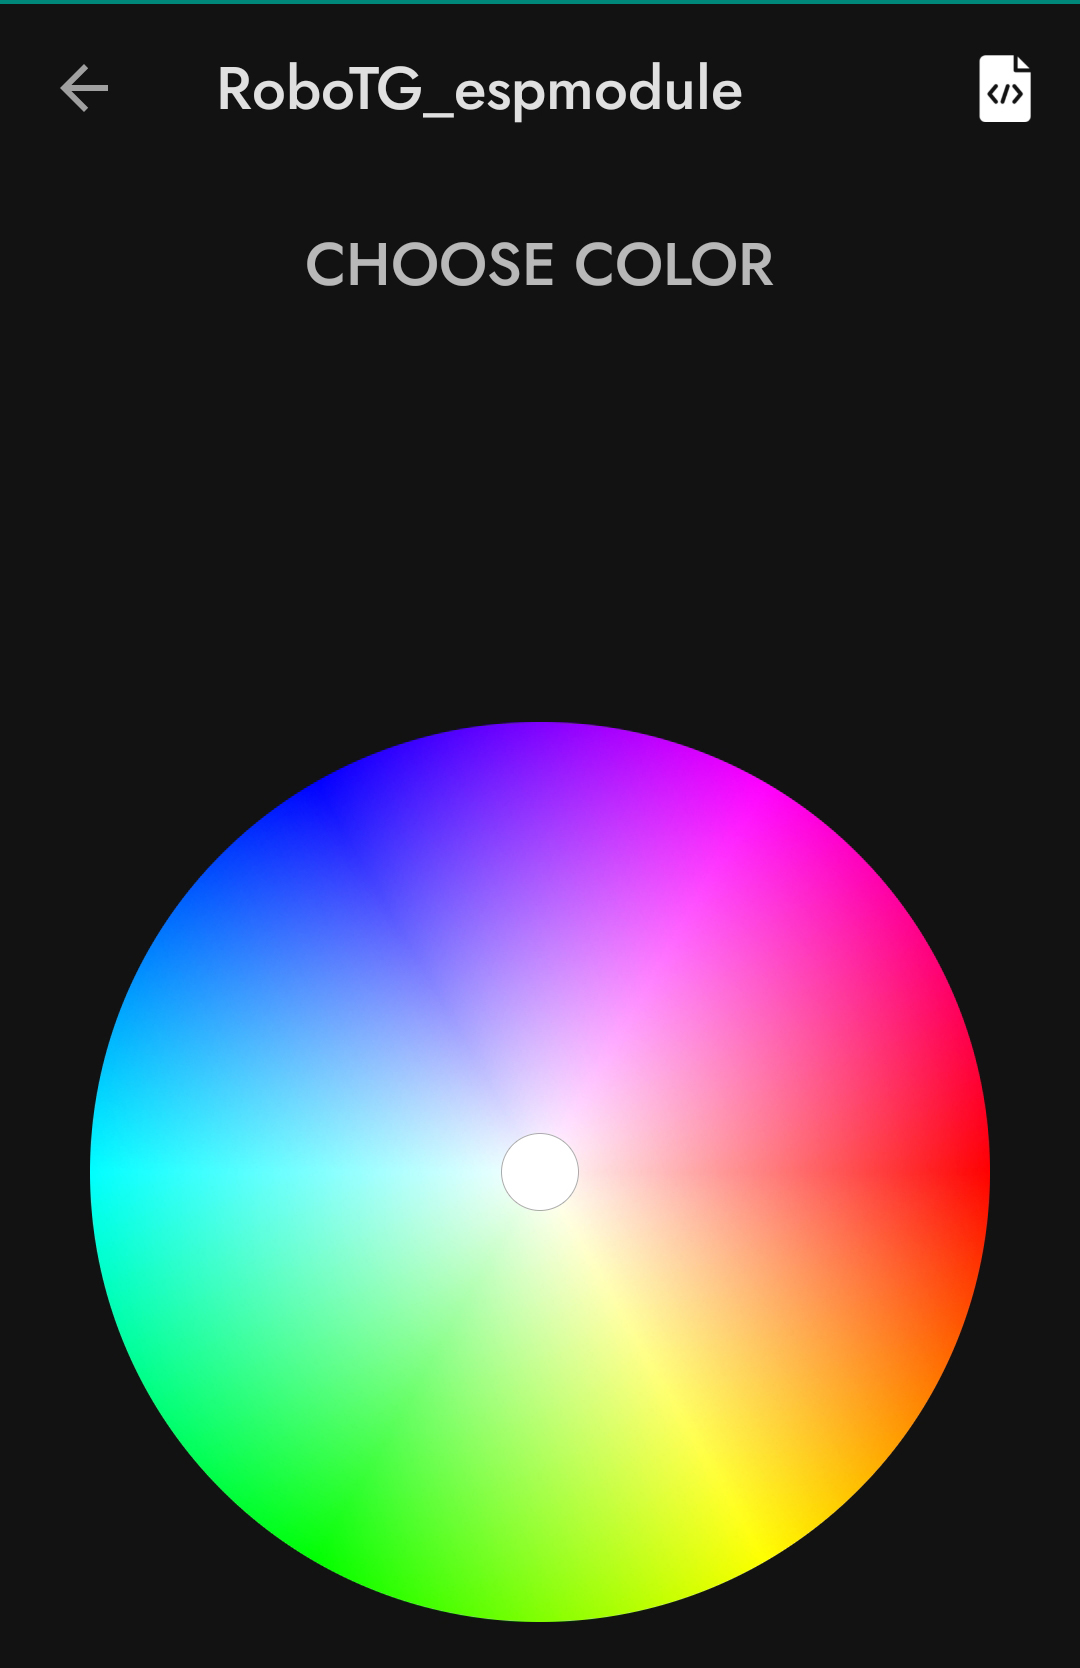
\includegraphics[width=0.40\textwidth]{figures/andriod_bluetooth_controller_hsl_model}
	\caption{Tela de controle RGB do aplicativo Arduino Bluetooth Controller}
	\label{arduino_bluetooth_controller_hsl_model}
\end{figure}

No modelo HSV,  figura  \ref{rbg_hsl_hsv}, 'H' significa "hue" ou matiz, e é um valor do angulo no modelo HSV, 'S' significa 'saturação' e corresponde a um valor de raio,
por último, 'V' é valor, que corresponde a uma terceira dimensão, que não aparece no modelo bidimensional disponível no aplicativo.
Exitem outros dois modelos parecidos que usam a mesma representação cilíndrica, HSL, e HSB, que possuem uma lógica semelhando ao HSV.


\begin{figure}[htb]
	\centering
	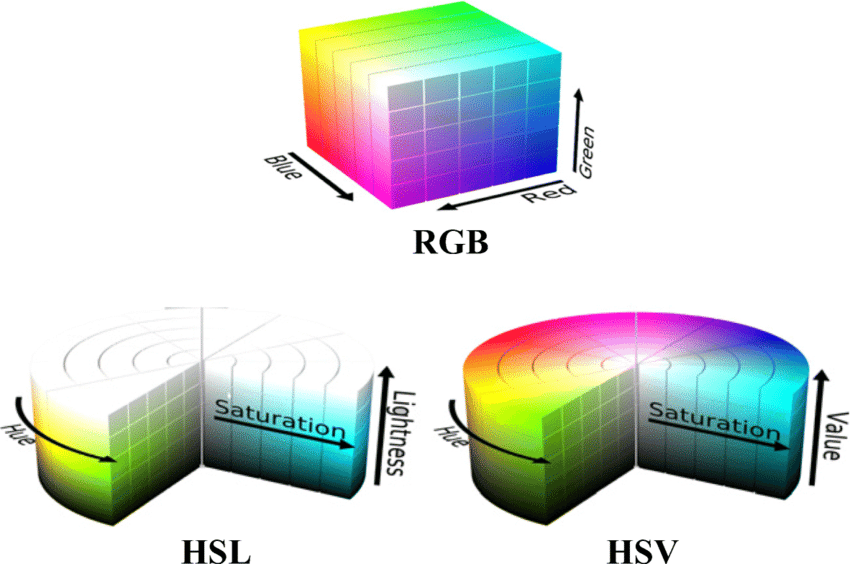
\includegraphics[width=0.6\textwidth]{figures/RBG_HSL_HSV}
	\caption{Modelos RGB, HSL e HSV \cite{rbg_hsl_hsv}}
	\label{rbg_hsl_hsv}
\end{figure}

\begin{figure}[htb]
	\centering
	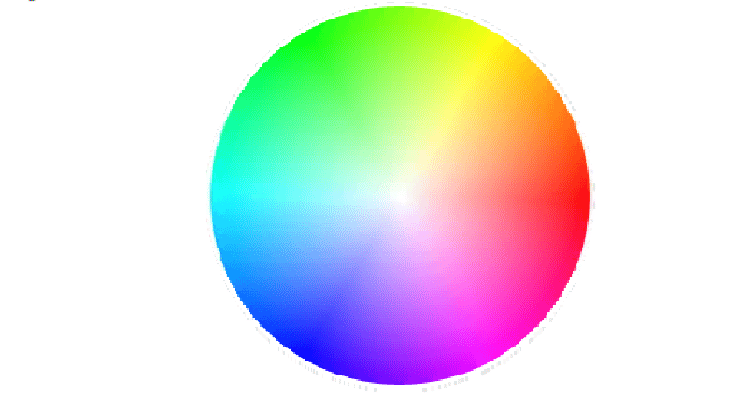
\includegraphics[width=0.8\textwidth]{figures/HSV}
	\caption{Modelo HSV bidimensional \cite{hsv_model}}
\end{figure}


O aplicativo retorna os valores em RGB, então usando um algorítimo que converte RGB para HSV e invertendo o eixo Y
é possível ter os valores de angulo e módulo de um vetor velocidade.
As imagens \ref{hsv_exemplo_1} e \ref{hsv_exemplo_2} possuem os seguintes valores de RGB, que aplicados no algorítimo de conversão geram os resultados no quadro \ref{HSV_resultado}
Facilmente podemos extrair informações de direção e magniture que podem ser usados para controlar o robô.

\begin{figure}[htb]
	\centering
	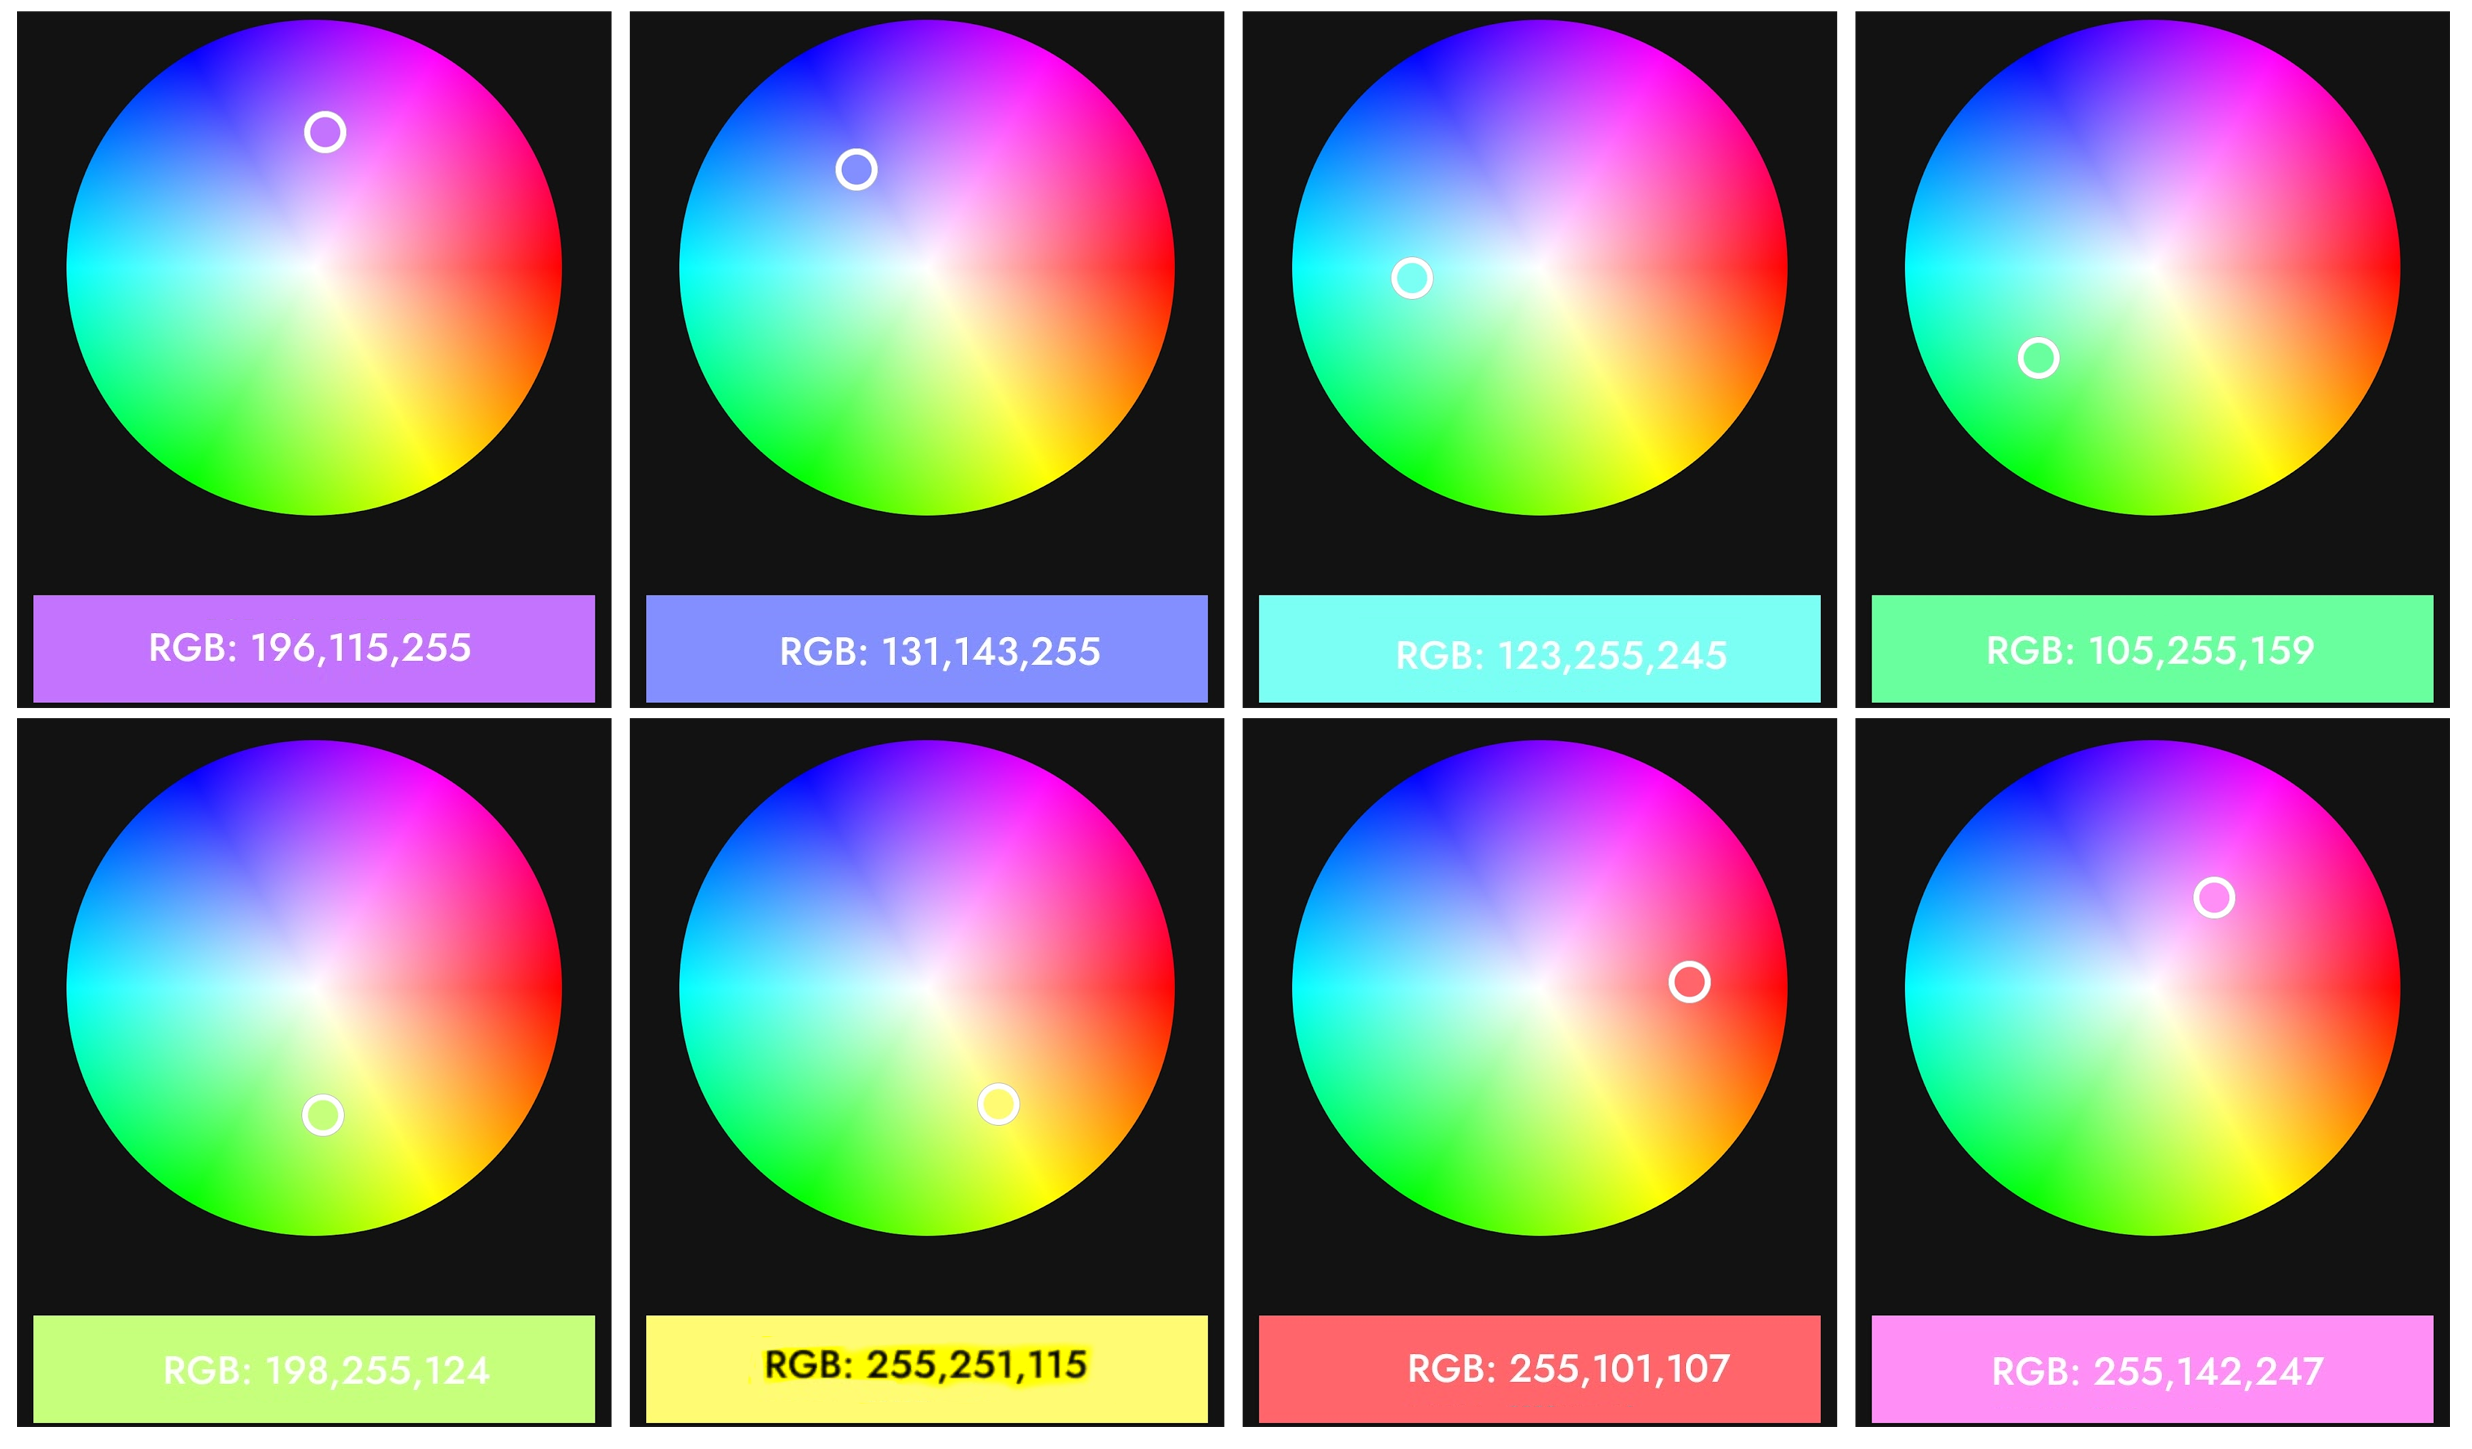
\includegraphics[width=1.0\textwidth]{figures/example_1_arduino_color}
	\caption{Modelo HSV bidimensional exemplos n1}
	\label{hsv_exemplo_1}
\end{figure}

\begin{figure}[htb]
	\centering
	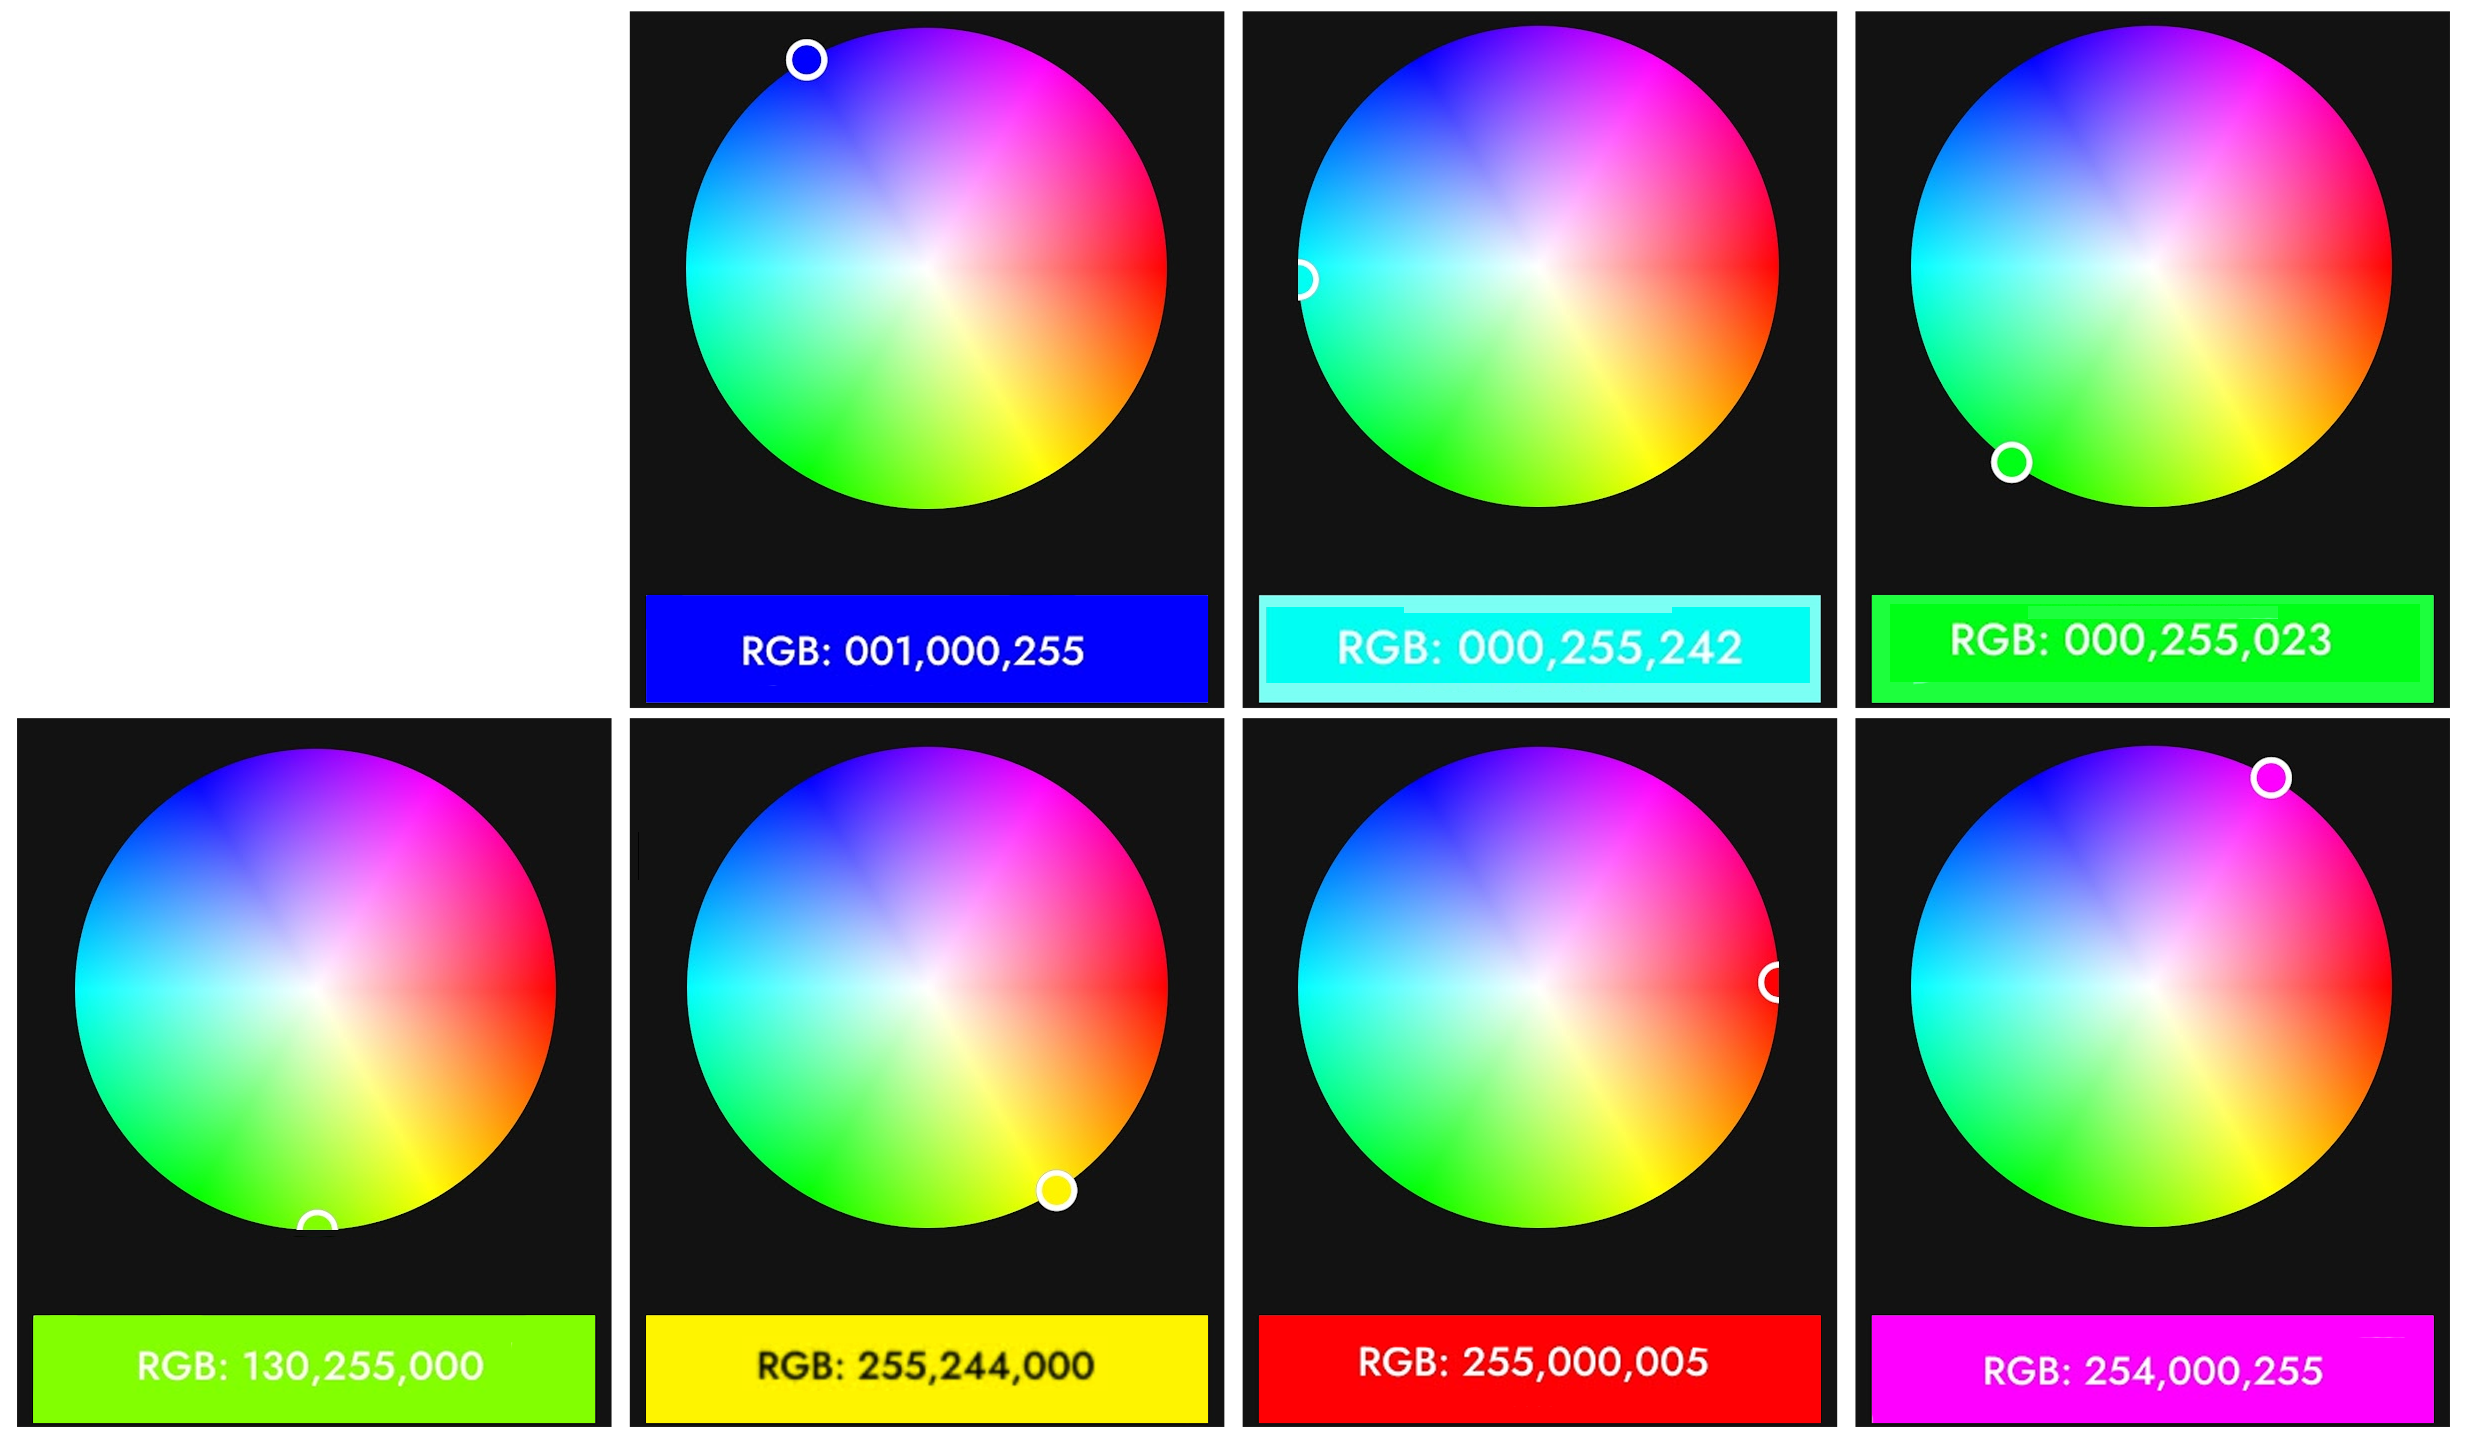
\includegraphics[width=1.0\textwidth]{figures/example_2_arduino_color}
	\caption{Modelo HSV bidimensional exemplos n2}
	\label{hsv_exemplo_2}
\end{figure}

\begin{quadro}[htb]
	\caption{\label{HSV_resultado}Resultado algoritmo}
		 \begin{tabular}{|c|c|c|}
			\hline
			\textbf{RGB} & \textbf{Ângulo} & \textbf{Magniture} \\ \hline
			196, 115, 255 & 275.0 & 54.9\% \\ \hline
			131, 143, 255 & 234.0 & 48.63\% \\ \hline
			123, 255, 245 & 175.0 & 51.76\% \\ \hline
			105, 255, 159 & 142.0 & 58.82\% \\ \hline
			198, 255, 124 & 86.0 & 51.37\% \\ \hline
			255, 251, 115 & 58.0 & 54.9\% \\ \hline
			255, 101, 107 & 358.0 & 60.39\% \\ \hline
			255, 142, 247 & 304.0 & 44.31\% \\ \hline
			001, 000, 255 & 240.0 & 100.0\% \\ \hline
			000, 255, 242 & 177.0 & 100.0\% \\ \hline
			000, 255, 023 & 125.0 & 100.0\% \\ \hline
			130, 255, 000 & 89.0 & 100.0\% \\ \hline
			255, 244, 000 & 57.0 & 100.0\% \\ \hline
			255, 000, 005 & 359.0 & 100.0\% \\ \hline
			254, 000, 255 & 300.0 & 100.0\% \\ \hline
		\end{tabular}
	\end{quadro}
